%%%%%%%%%%%%%%%%%%%%%%%%%%%%%%%%%%%%%%%%%%%%%%%%%%%%%%
% A Beamer template for University of Wollongong     %
% Based on THU beamer theme                          %
% Author: Qiuyu Lu                                   %
% Date: July 2024                                    %
% LPPL Licensed.                                     %
%%%%%%%%%%%%%%%%%%%%%%%%%%%%%%%%%%%%%%%%%%%%%%%%%%%%%%
% Customized for Sharif University of Technology     %
%%%%%%%%%%%%%%%%%%%%%%%%%%%%%%%%%%%%%%%%%%%%%%%%%%%%%%


\documentclass[serif, aspectratio=169]{beamer}
%\documentclass[serif]{beamer}  % for 4:3 ratio
\usepackage[T1]{fontenc} 
\usepackage{fourier} % see "http://faq.ktug.org/wiki/uploads/MathFonts.pdf" for other options
\usepackage{hyperref}
\usepackage{latexsym,amsmath,xcolor,multicol,booktabs,calligra}
\usepackage{graphicx,pstricks,listings,stackengine}
\usepackage{lipsum}
\usepackage{booktabs}
%\usepackage{geometry}
\usepackage{tabularx}
\author{Ali Sharifi-Zarchi}
\title{Machine Learning (CE 40717)}
\subtitle{Fall 2024}
\institute{
    CE Department \\
    Sharif University of Technology
}
%\date{\small \today}
% \usepackage{UoWstyle}
\usepackage{SUTstyle}

% defs
\def\cmd#1{\texttt{\color{red}\footnotesize $\backslash$#1}}
\def\env#1{\texttt{\color{blue}\footnotesize #1}}
\definecolor{deepblue}{rgb}{0,0,0.5}
\definecolor{deepred}{RGB}{153,0,0}
\definecolor{deepgreen}{rgb}{0,0.5,0}
\definecolor{halfgray}{gray}{0.55}

\lstset{
    basicstyle=\ttfamily\small,
    keywordstyle=\bfseries\color{deepblue},
    emphstyle=\ttfamily\color{deepred},    % Custom highlighting style
    stringstyle=\color{deepgreen},
    numbers=left,
    numberstyle=\small\color{halfgray},
    rulesepcolor=\color{red!20!green!20!blue!20},
    frame=shadowbox,
}

\begin{document}

\begin{frame}
    \titlepage
    \vspace*{-0.6cm}
    \begin{figure}[htpb]
        \begin{center}
            
\includegraphics[keepaspectratio, scale=0.25]{pic/sharif-main-logo.png}
        \end{center}
    \end{figure}
\end{frame}

\begin{frame}    
\tableofcontents[sectionstyle=show,
subsectionstyle=show/shaded/hide,
subsubsectionstyle=show/shaded/hide]
\end{frame}

\section{Optimization}

\begin{frame}{Optimization Problem}
    \begin{itemize}
        \item \textbf{Goal}: Find the value of $x$ where $f(x)$ is at a \textbf{minimum} or \textbf{maximum}.
        \item In neural networks, we aim to minimize \textbf{prediction error} by finding the optimal weights $w^*$:
    \end{itemize}
    
    \[
    w^* = \arg\min_{w} J(w)
    \]
    
    \begin{itemize}
        \item Simply put: determine the \textbf{direction to step} that will quickly \textbf{reduce loss}.
    \end{itemize}
    
    % \begin{figure}[h]
    %     \centering
    %     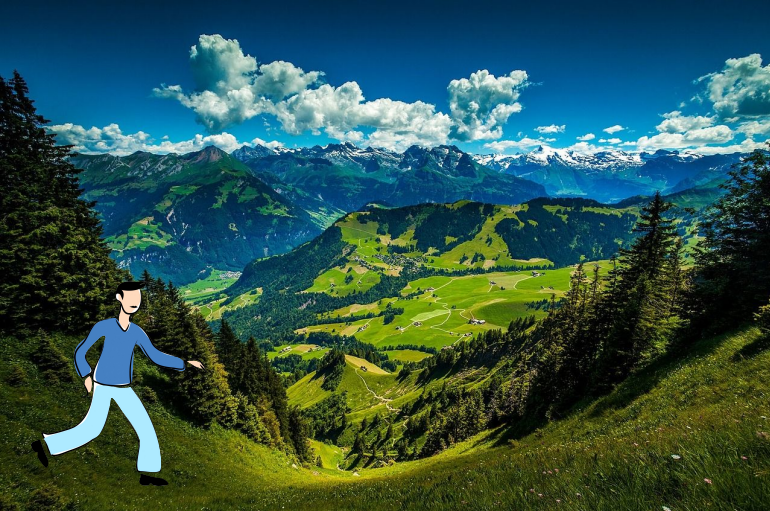
\includegraphics[width=0.3\linewidth]{pic/downhill_feifei_rouhan.png}
    %     \caption{Which way is downhill? (CS231n, Stanford)}
    % \end{figure}
\end{frame}

\begin{frame}{Convexity and Optimization}
\begin{minipage}{0.6\linewidth}
    \begin{itemize}
        \item \textbf{Convex Functions}:
        \begin{itemize}
            \item A function is \textbf{convex} if any line segment between points on the curve lies \textbf{above or on} the curve.\\
            \item Convex functions are easier to optimize, as they have a single \textbf{global minimum}.\\
            \item Numerical methods like \textbf{Gradient Descent} are guaranteed to reach the global minimum in convex functions.
        \end{itemize}
    \end{itemize}
\end{minipage}%
\begin{minipage}{0.3\linewidth}
    \begin{figure}[h]
        \centering
        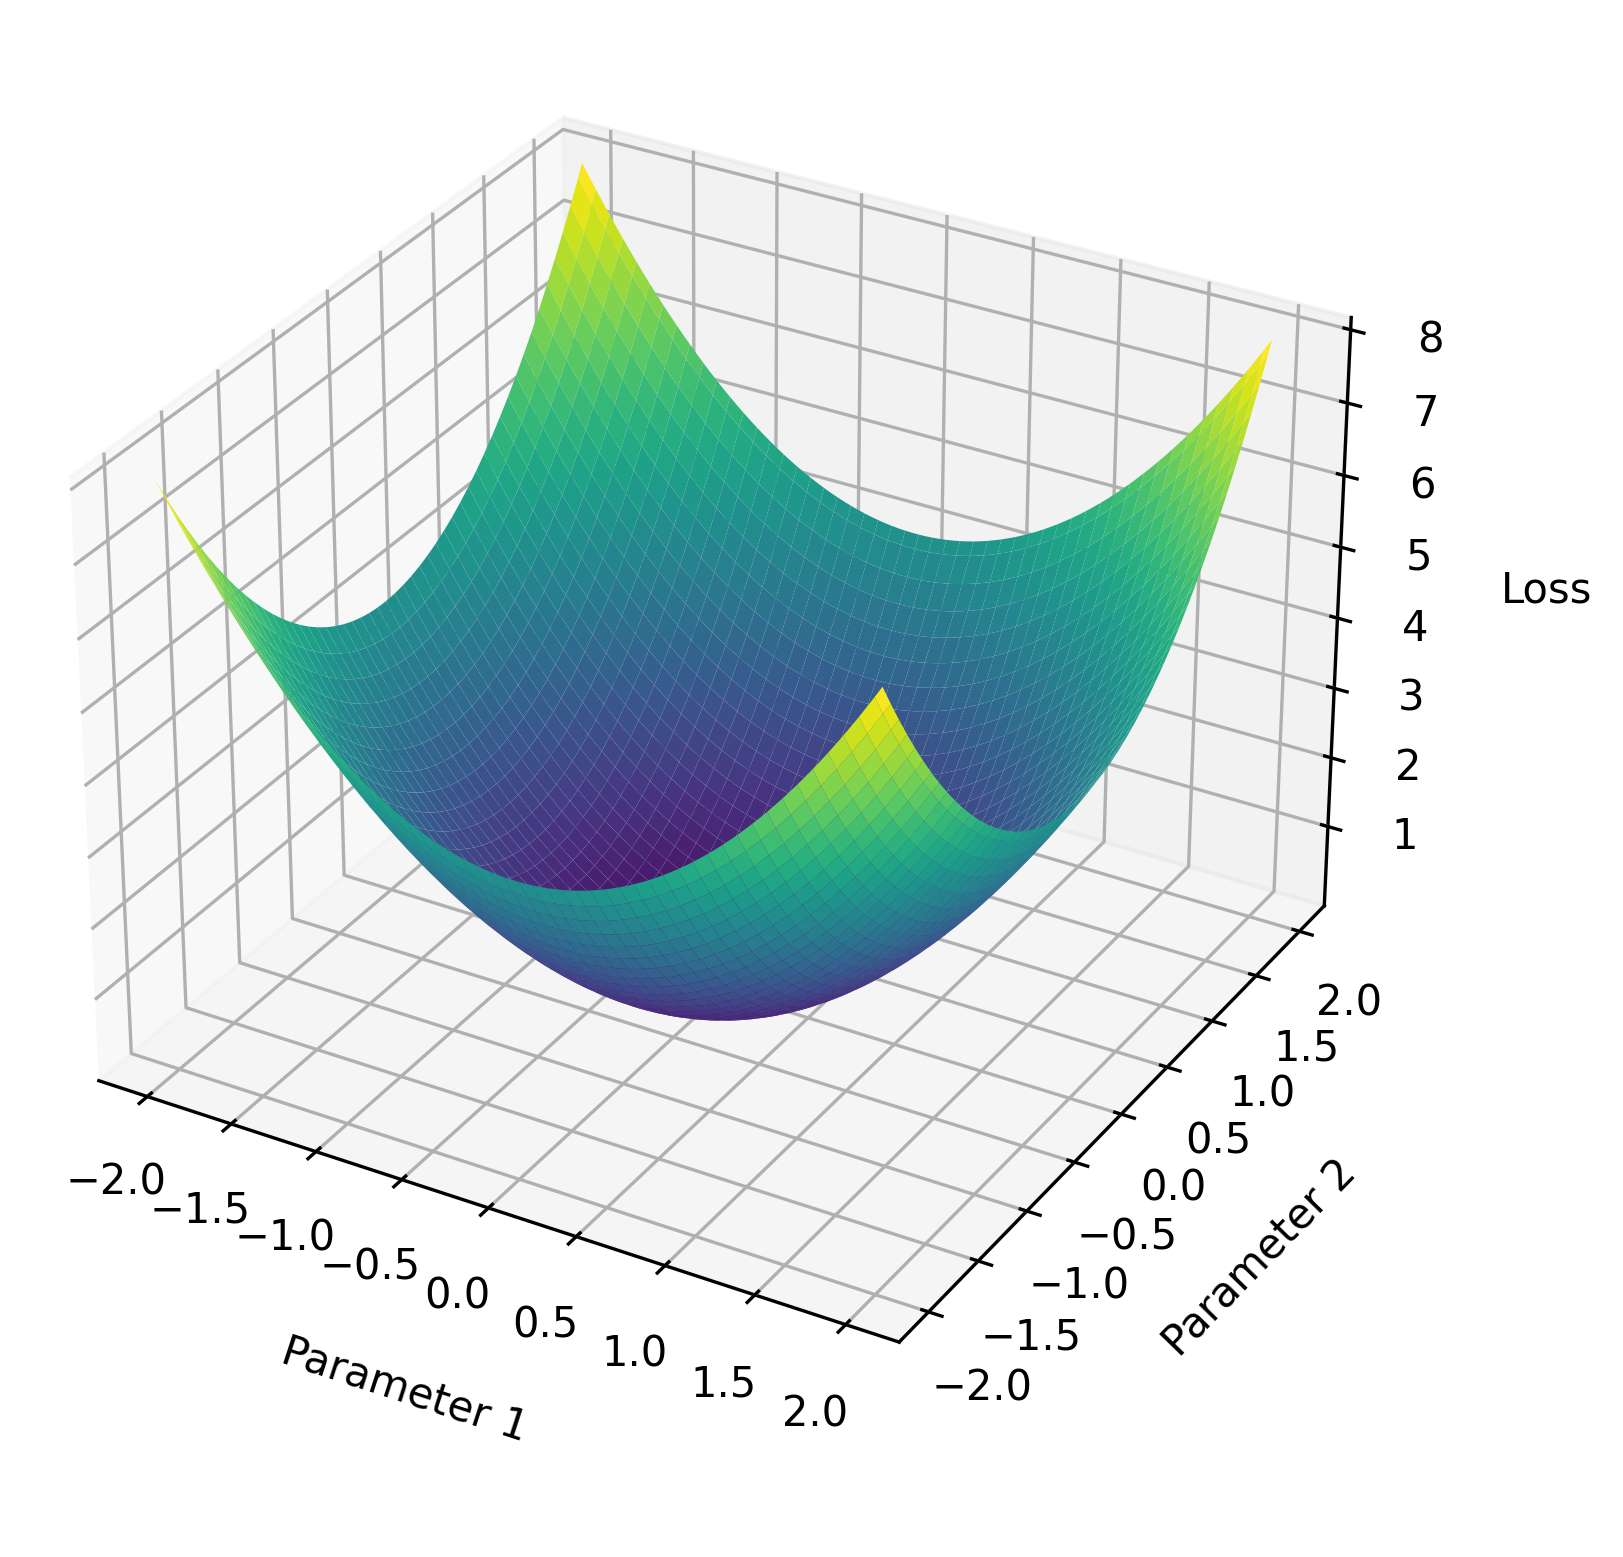
\includegraphics[height=0.7\textheight]{pic/loss_convex.jpg}
        \caption{\footnotesize Example of convex function (bowl shape)}
    \end{figure}
\end{minipage}
\end{frame}

\begin{frame}{Non-Convex Functions and Challenges}
\begin{minipage}{0.65\linewidth}
    \begin{itemize}
        \item \textbf{Non-Convex Functions}:
        \begin{itemize}
            \item Characterized by multiple \textbf{local minima} and \textbf{saddle points}.
            \item \textbf{Global Minimum}: Overall lowest point.
            \item \textbf{Local Minimum}: Lower than nearby points, but not the lowest overall.
            \item \textbf{Saddle Points}: Regions where the gradient is close to zero but can increase or decrease in other directions.
        \end{itemize}
        \item Finding the \textbf{global minimum} is more complex in non-convex functions.
    \end{itemize}
\end{minipage}%
\begin{minipage}{0.25\linewidth}
    \begin{figure}[h]
        \centering
        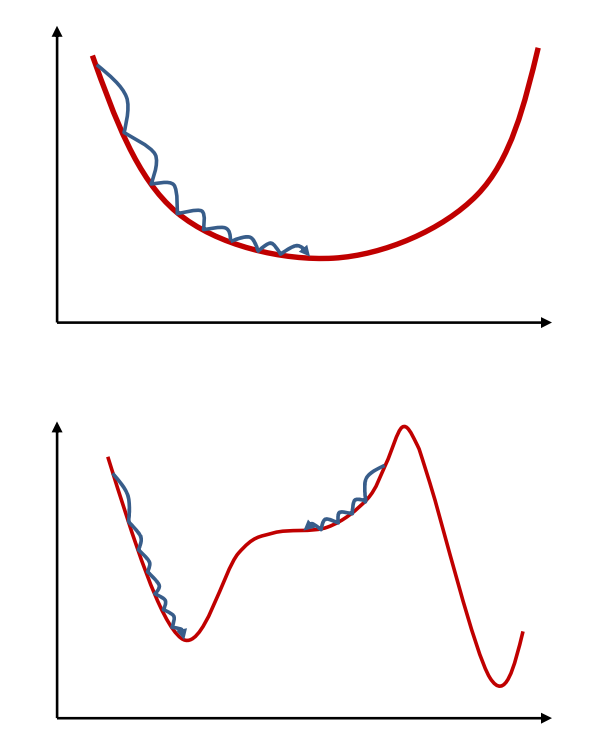
\includegraphics[height=0.65\textheight]{pic/convex_nonconvex.png}
        \caption{\footnotesize Convex (top) vs. Non-Convex (bottom) functions. Source: (CMU, 11-785)}
    \end{figure}
\end{minipage}
\end{frame}

\section{The Loss Surface}
\begin{frame}{Loss Surface Definition}
\begin{minipage}{0.6\linewidth}
    \begin{itemize}
        \item The \textbf{loss surface} shows how error changes based on network weights.
        \item For neural networks, the loss surface is typically \textbf{non-convex} due to multiple layers, nonlinear activations, and complex parameter interactions, resulting in \textbf{multiple local minima} and \textbf{saddle points}.
        \item In large networks, most local minima yield similar error values close to the \textbf{global minimum}; this is less true in smaller networks.
    \end{itemize}
\end{minipage}%
\begin{minipage}{0.3\linewidth}
    \begin{figure}[h]
        \centering
        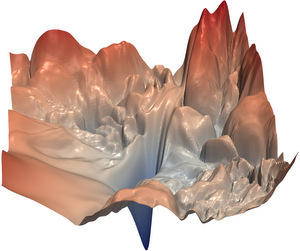
\includegraphics[height=0.6\textheight]{pic/resnet56_noshort_small.jpg}
        \caption{\footnotesize Loss surface of ResNet56. Source: \href{https://github.com/tomgoldstein/loss-landscape}{GitHub: Loss Landscape}}
    \end{figure}
\end{minipage}
\end{frame}

\begin{frame}{Loss Optimization}
    \begin{itemize}
        \item \textbf{Goal}: How can we optimize a non-convex loss function effectively?
        \item \textbf{Gradient Descent}:
        \begin{itemize}
            \item This method identifies the \textbf{steepest descent direction} to guide the optimization process.
        \end{itemize}
        \item \textbf{Newton's Method}:
        \begin{itemize}
            \item This method looks for \textbf{critical points} where the derivative \( f'(x) = 0 \), which may indicate minima, maxima, or saddle points.
            \item Newton's Method uses the second derivative (Hessian) to adjust step sizes, which can lead to faster convergence compared to Gradient Descent.
        \end{itemize}
    \end{itemize}
\end{frame}

\section{Gradient Descent}
\begin{frame}{Gradient Descent Overview}
    \begin{itemize}
        \item \textbf{Gradient Descent}: As mentioned earlier in this course, Gradient Descent is an iterative method to minimize error by updating weights in the direction of the \textbf{negative gradient}:
        \[
        w_{t+1} = w_t - \eta \nabla J(w_t)
        \]
        where $\eta$ is the \textbf{learning rate}.
    \end{itemize}
    \begin{itemize}
        \item \textbf{Types of Gradient Descent}:
        \begin{itemize}
            \item \textbf{Batch}: Full dataset for stable but slow updates.
            \item \textbf{Stochastic (SGD)}: One data point for fast, noisy updates.
            \item \textbf{Mini-Batch}: Small batches, balancing speed and stability.
        \end{itemize}
    \end{itemize}
\end{frame}

\begin{frame}{Problems with Gradient Descent}
    \begin{itemize}
        \item \textbf{High Variability (SGD)}: Quick in steep directions but slow in shallow ones, causing \textbf{jitter and slow progress}.
        \item \textbf{Local Minima and Saddle Points}: Risk of \textbf{sub-optimal solutions} or long convergence times in flat regions.
        \item \textbf{Noisy Updates}: Using individual points or mini-batches introduces noise, affecting stable convergence.
    \end{itemize}
    \vfill
    \begin{minipage}{0.5\linewidth}
        \begin{figure}[h]
        \centering
        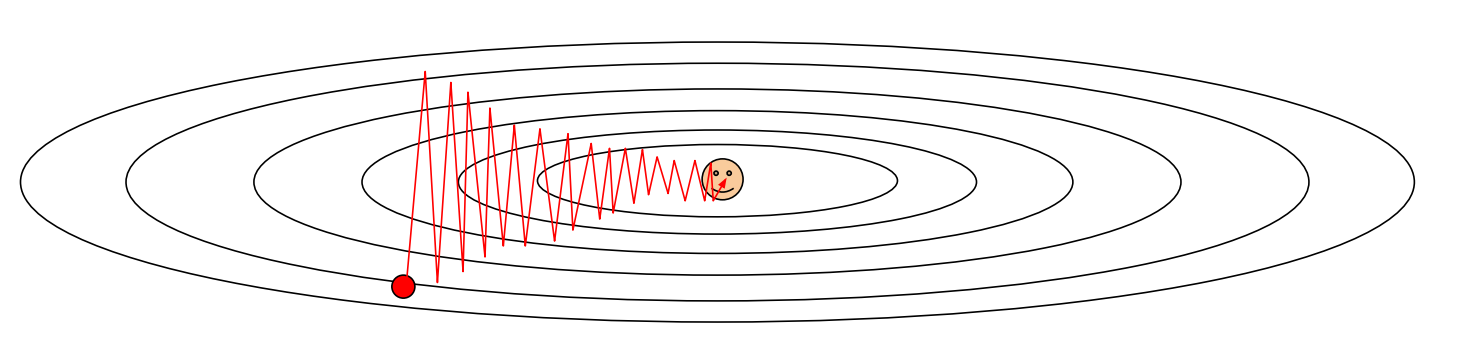
\includegraphics[width=1\linewidth]{pic/sgd_stanford.png}
        \caption{\footnotesize SGD Variability (CS231n, Stanford)}
        \end{figure}
    \end{minipage}%
    \hfill
    \begin{minipage}{0.5\linewidth}
        \begin{figure}
            \centering
            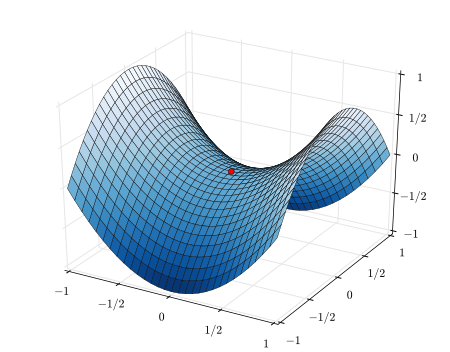
\includegraphics[width=0.5\linewidth]{pic/saddle_wiki.png}
            \caption{\footnotesize Saddle Point. Source: \href{https://en.wikipedia.org/wiki/Saddle_point}{Wikipedia}}
        \end{figure}
    \end{minipage}
\end{frame}

\section{Momentum}
\begin{frame}{Problem Definition}
    \begin{minipage}{0.6\textwidth}
    \begin{itemize}
        \item \textbf{Objective}: \textbf{Enhance} the vanilla Gradient Descent algorithm to improve convergence and stability.
        \item \textbf{Challenges}:
        \begin{itemize}
            \item Selecting \textbf{an appropriate learning rate} is crucial to avoid slow convergence and getting stuck in local minima.
        \end{itemize}
        \item \textbf{Proposed Solution}:
        \begin{itemize}
            \item Instead of testing multiple learning rates, incorporate \textbf{Momentum} to adaptively adjust the learning rate based on oscillations:
            \begin{itemize}
                \item Increase steps in stable directions.
                \item Decrease steps in oscillating directions.
            \end{itemize}
        \end{itemize}
    \end{itemize}
    \end{minipage}%
    \begin{minipage}{0.3\textwidth}
        \begin{figure}[h]
            \centering
            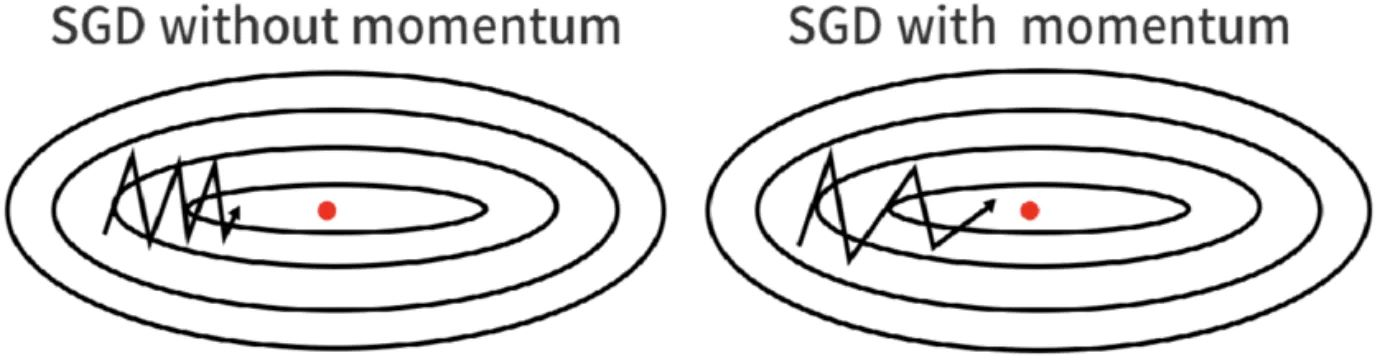
\includegraphics[height=0.2\textheight]{pic/momentum_paperswithcode.jpg}
            \caption{\footnotesize Momentum smooths oscillations and accelerates progress. Source: \href{https://paperswithcode.com/method/sgd-with-momentum}{Papers with Code}}
        \end{figure}
    \end{minipage}
\end{frame}

\begin{frame}{Introduction to Momentum in Optimization}
    \begin{itemize}
        \item \textbf{Origin of Momentum}: 
        \begin{itemize}
            \item Inspired by Newtonian physics, momentum in optimization uses \textbf{the concept of velocity in motion}, accumulating gradient history to smooth the learning trajectory, akin to an object moving based on past inertia.
            \item Initially introduced to tackle challenges in gradient descent, where \textbf{inconsistent gradients or noisy updates} lead to erratic and slow convergence.
        \end{itemize}
        
        \item \textbf{Purpose of Momentum}: 
        \begin{itemize}
            \item \textbf{Dampens Oscillations}: Utilizes prior gradients to minimize oscillations along steep or erratic regions, resulting in a smoother and more stable path.
            \item \textbf{Speeds Up Convergence}: Particularly effective in narrow valleys or flat regions, where standard gradient descent may struggle or oscillate, causing slow progress.
        \end{itemize}
        
        % \item \textbf{Mechanism}: 
        % \begin{itemize}
        %     \item Achieves improvements by adding a "velocity" term to gradient descent, facilitating consistent directional movement and balancing update sizes for faster and more reliable convergence.
        % \end{itemize}
    \end{itemize}
\end{frame}

% \begin{frame}{How Momentum Accelerates Learning}
%     \begin{itemize}
%         \item In momentum-based optimization, updates are influenced by a weighted combination of the current gradient and previous updates.
%         \item \textbf{Why Use Momentum?}
%         \begin{itemize}
%             \item \textbf{Reduces Oscillations}: Momentum softens oscillations along steeper directions while preserving progress in directions with smaller gradients, resulting in a balanced path.
%             \item \textbf{Increases Efficiency}: By "accelerating" updates in directions of consistent gradient descent, momentum minimizes unnecessary steps and decreases overall convergence time.
%         \end{itemize}
%     \end{itemize}
% \end{frame}

\subsection{First Moment (Momentum)}
\begin{frame}{First Moment (Momentum)}
    \begin{itemize}
        \item \textbf{Definition}: The first moment, \( m_t \), represents a moving average of past gradients. It builds "velocity" that propels learning in a consistent direction.
        \item \textbf{Update Rule}:
        \[
        m_{t+1} = \beta_1 m_t + (1 - \beta_1) \nabla_w J(w_t)
        \]
        \[
        w_{t+1} = w_t - \eta m_{t+1}
        \]
        where:
        \begin{itemize}
            \item \( \beta_1 \): Decay rate, usually 0.9 or 0.99, which controls the weight of past gradients.
            \item \( \eta \): Learning rate.
        \end{itemize}
        \item \textbf{Why Use First Momentum?}
        \begin{itemize}
            \item Inspired by the idea of rolling momentum, it smooths and accelerates learning by sustaining direction from prior gradients.
            \item This type of momentum is ideal for traversing narrow valleys or regions where standard gradient descent would oscillate.
        \end{itemize}
    \end{itemize}
\end{frame}

\begin{frame}{Example of First Moment}
    \begin{minipage}{0.45\linewidth}
        \begin{figure}
            \centering
            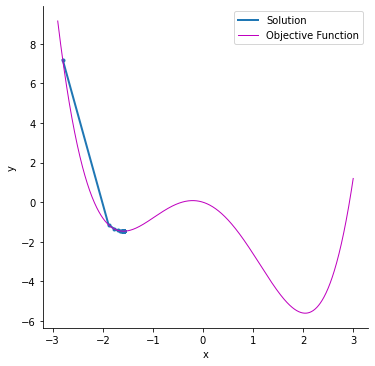
\includegraphics[width=0.75\linewidth]{pic/Without_momentum.png}
            \caption{\footnotesize Stochastic gradient descent without momentum stops at a local minimum. Source: Akash Ajagekar (SYSEN 6800 Fall 2021)}
        \end{figure}
    \end{minipage}%
    \begin{minipage}{0.45\linewidth}
        \begin{figure}
            \centering
            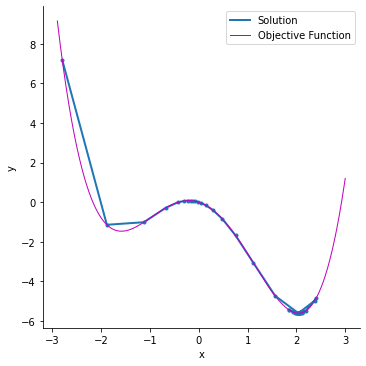
\includegraphics[width=0.75\linewidth]{pic/With_momentum.png}
            \caption{\footnotesize Stochastic gradient descent with momentum stops at the global minimum. Source: Akash Ajagekar (SYSEN 6800 Fall 2021)}
        \end{figure}
    \end{minipage}
\end{frame}

\subsection{Second Moment (Variance)}
\begin{frame}{Second Moment (Variance)}
    \begin{itemize}
        \item \textbf{Definition}: The second moment, \( v_t \), represents the moving average of squared gradients. It measures the gradient magnitude over time.
        \item \textbf{Update Rule}:
        \[
        v_{t+1} = \beta_2 v_t + (1 - \beta_2) (\nabla_w J(w_t))^2
        \]
        \[
        w_{t+1} = w_t - \frac{\eta}{\sqrt{v_{t+1} + \epsilon}} \nabla_w J(w_t)
        \]
        where:
        \begin{itemize}
            \item \( \beta_2 \): Decay rate for variance (usually 0.99 or 0.999).
            \item \( \epsilon \): Small constant to prevent division by zero.
        \end{itemize}
        \item \textbf{Why Use Second Momentum?}
        \begin{itemize}
            \item Adjusts step size based on gradient magnitude, preventing large steps when gradients are large and accelerating learning when they are small.
        \end{itemize}
    \end{itemize}
\end{frame}

\begin{frame}{Moment Bias Correction}
    \begin{itemize}
        \item \textbf{Problem}: When we start training, both $m_{t}$ and $v_{t}$ are initialized to zero, causing their estimates to be \textbf{biased toward zero in the early steps}, especially when gradients are small.
        \item \textbf{Solution}: We use bias-corrected versions of $m_{t}$ and $v_{t}$ to address this:
        \[\hat{m}_{t} = \frac{m_{t}}{1 - \beta_1^{t}}, \quad 
        \hat{v}_{t} = \frac{v_{t}}{1 -\beta_2^{t}}\]
        \item These corrections compensate for the bias by scaling $m_{t}$ and $v_{t}$ upward, especially in the early steps when $t$ is small, ensuring more accurate estimates of the moments.
    \end{itemize}
\end{frame}

\subsection{Adam: Adaptive Moment Estimation}
\begin{frame}{Introduction to Adam Optimizer}
    \begin{itemize}
        \item \textbf{Origin and Purpose}: 
        \begin{itemize}
            \item Proposed in 2014 by Diederik Kingma and Jimmy Ba, Adam (Adaptive Moment Estimation) addresses key limitations in earlier optimization methods by combining aspects of \textbf{momentum} and \textbf{adaptive learning rates}.
            \item Adam is designed to handle sparse gradients and noisy updates by adjusting the learning rate for each parameter based on historical gradients.
        \end{itemize}
        \item \textbf{Core Idea}:
        \begin{itemize}
            \item Adam optimizes by maintaining two moving averages — the \textbf{first moment (mean of gradients)} and the \textbf{second moment (variance of gradients)} — allowing it to \textbf{adapt learning rates for each parameter individually}.
        \end{itemize}
    \end{itemize}
\end{frame}

\begin{frame}{Adam’s Adaptive Learning Rate Mechanism}
    \begin{itemize}
        \item \textbf{Why Adaptive Rates?}
        \begin{itemize}
            \item Unlike traditional SGD, Adam adapts the learning rate for \textbf{each parameter} based on recent gradient magnitudes.
            \item \textbf{Large gradients} lead to \textbf{reduced} update sizes, while \textbf{smaller gradients} allow \textbf{larger} updates, balancing convergence speed and stability.
        \end{itemize}
        \item \textbf{Moment Tracking}
        \begin{itemize}
            \item The \textbf{first moment} ($m_t$) tracks the mean of gradients to provide momentum.
            \item The \textbf{second moment} ($v_t$) tracks squared gradients, enabling Adam to normalize updates and prevent sudden changes in direction.
        \end{itemize}
    \end{itemize}
\end{frame}

\begin{frame}{Mathematical Formulation of Adam}
    \begin{itemize}
        \item \textbf{Adam Update Rules}:
        \begin{itemize}
            \item First moment estimate:
            \[
            m_{t+1} = \beta_1 m_t + (1 - \beta_1) \nabla_w J(w_t)
            \]
            \item Second moment estimate:
            \[
            v_{t+1} = \beta_2 v_t + (1 - \beta_2) (\nabla_w J(w_t))^2
            \]
            \item Bias-corrected moments to address initialization bias:
            \[
            \hat{m}_{t+1} = \frac{m_{t+1}}{1 - \beta_1^{t+1}}, \quad 
            \hat{v}_{t+1} = \frac{v_{t+1}}{1 - \beta_2^{t+1}}
            \]
            \item Update step for parameter \( w_t \):
            \[
            w_{t+1} = w_t - \eta \frac{\hat{m}_{t+1}}{\sqrt{\hat{v}_{t+1}} + \epsilon}
            \]
        \end{itemize}
        % where \(\beta_1\), \(\beta_2\) are decay rates, and \(\epsilon\) is a small constant to prevent division by zero.
    \end{itemize}
\end{frame}

\begin{frame}{Adam Pseudo-code}
    \begin{figure}
        \centering
        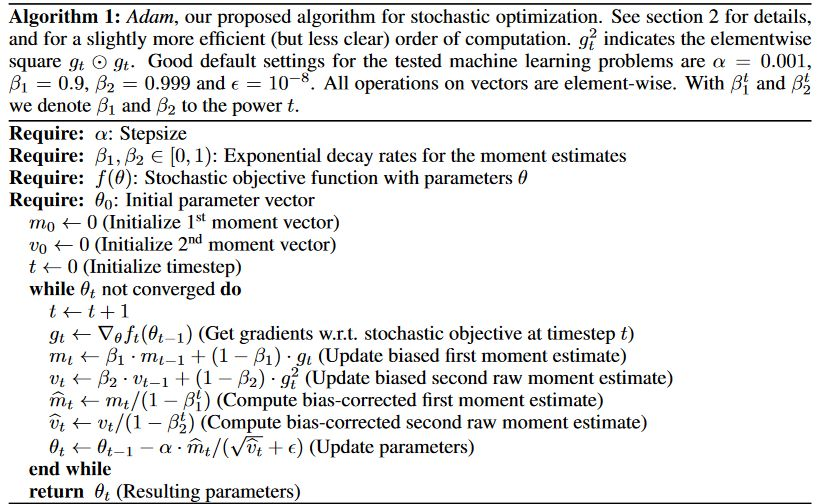
\includegraphics[width=0.7\linewidth]{adam_pseudocode.jpg}
        \caption{\footnotesize Adam Pseudo-code. Source: kingma2014adam}

    \end{figure}
\end{frame}

\begin{frame}{Adam Visualization}
\begin{figure}
    \centering
    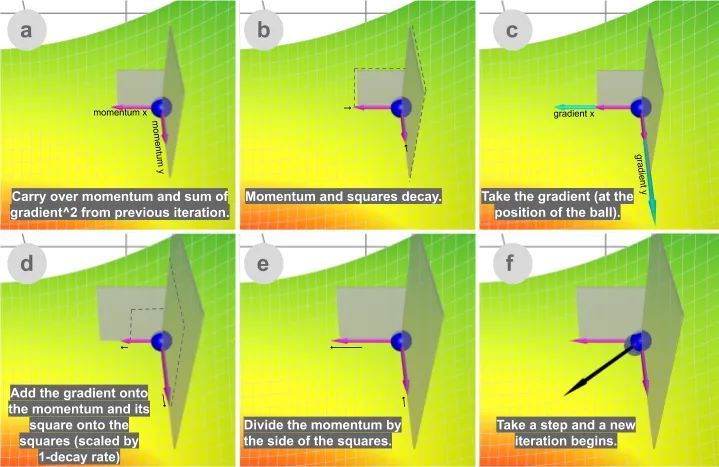
\includegraphics[width=0.65\linewidth]{pic/adam_towardsdatascience.jpg}
    \caption{\footnotesize Step-by-step illustration of Adam descent. Source: \href{https://towardsdatascience.com/a-visual-explanation-of-gradient-descent-methods-momentum-adagrad-rmsprop-adam-f898b102325c}{Towards Data Science}}
\end{figure}

\end{frame}

\begin{frame}{Comparison of Momentum Methods}
    \centering
    \begin{figure}
        \centering
        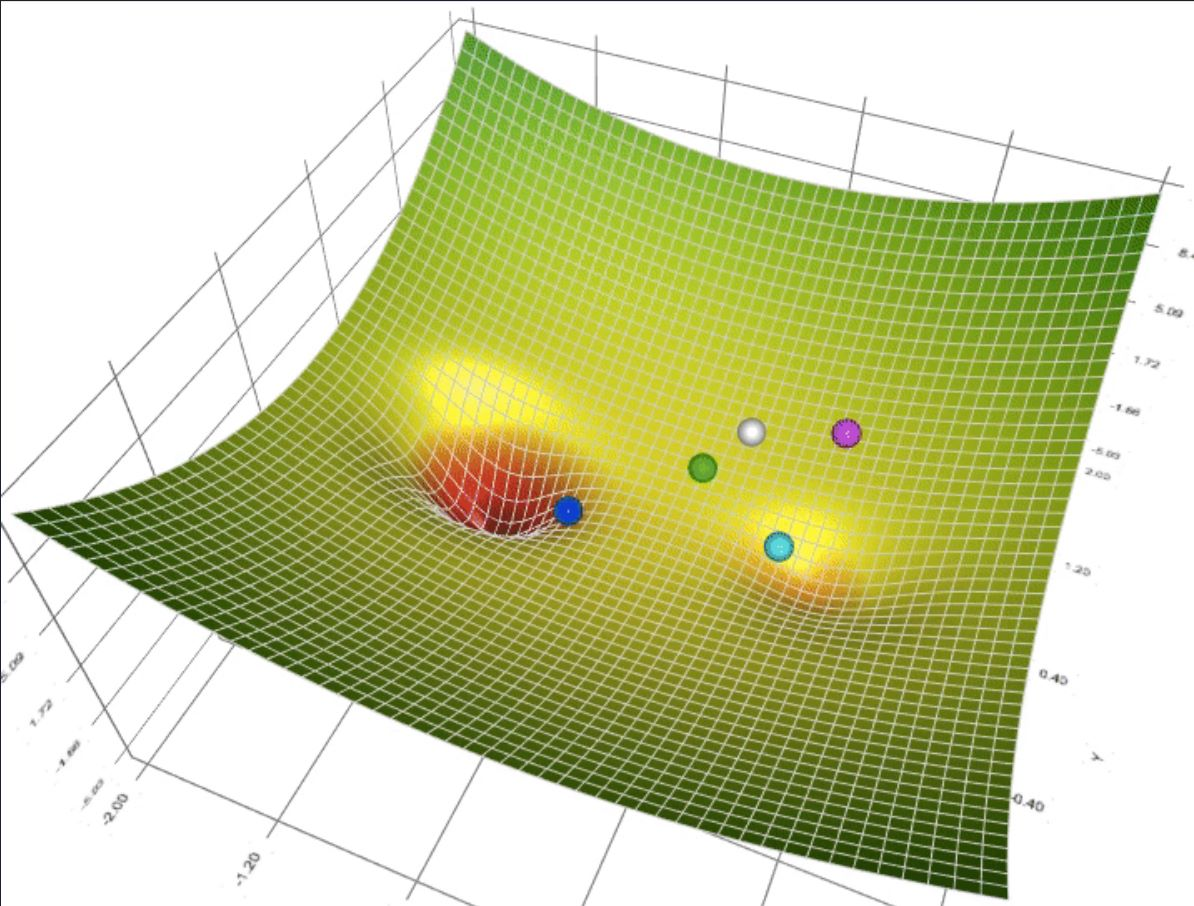
\includegraphics[width=0.5\linewidth]{pic/comparison.jpg}
        \caption{\footnotesize Comparison of 5 gradient descent methods on a surface: gradient descent (cyan), momentum (magenta), AdaGrad (white), RMSProp (green), Adam (blue). Left well is the global minimum; right well is a local minimum. Source: \href{https://towardsdatascience.com/a-visual-explanation-of-gradient-descent-methods-momentum-adagrad-rmsprop-adam-f898b102325c}{Towards Data Science}}
    \end{figure}
\end{frame}

\section{Newton's optimization Method}
\subsection{Newton's Method}
\begin{frame}{Newton's Method}
\begin{itemize}
    \item Newton method is originally intended to \textbf{find the root(s)} of an equation.
    \item \textbf{Example:} for the equation $x^2 - 1 = 0$, we can find the roots by decomposing $(x-1)(x+1)=0$ which gives $x=1, x=-1$
    \item \textbf{But, what about complex equations?}
    \begin{itemize}
        \item We can use \textbf{numerical method} to find the root of an equation, one of them is by using \textbf{Newton’s method}
    \end{itemize}
\end{itemize}
\end{frame}

\begin{frame}{Definition}
\begin{minipage}{0.55\linewidth}
\begin{itemize}
    \item \textbf{Objective:} Derive Newton’s method by finding the tangent line of \( f(x) \) at \( x_0 \).
    \item \textbf{Tangent Line Equation:} Given a point \( x_0 \) where \( f(x_0) \neq 0 \), the tangent line at \( x_0 \) is:
    \[
    y = mx_0 + c
    \]
    \item \textbf{Gradient:} The slope \( m \) matches the derivative of \( f(x) \) at \( x_0 \):
    \[
    m = f'(x_0)
    \]
\end{itemize}
\end{minipage}%
\begin{minipage}{0.35\linewidth}
    \begin{figure}
        \centering
        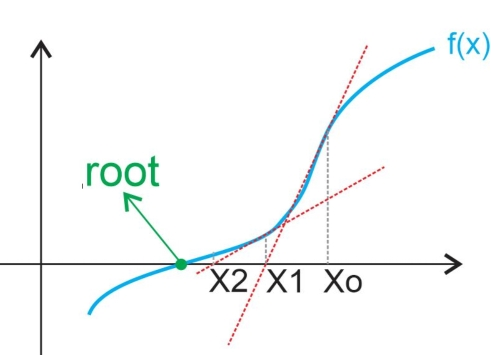
\includegraphics[width=1\linewidth]{pic/newton_raphson_ardianumam.jpg}
        \caption{\footnotesize Finding root location by using Newton’s method. Source: \href{https://ardianumam.wordpress.com}{Ardian Umam's Blog}}
    \end{figure}
\end{minipage}
\end{frame}

\begin{frame}{Formulating the Tangent Line}
\begin{itemize}
    \item \textbf{Finding \( c \) :} Substitute \( (x_0, f(x_0)) \) into \( y = mx + c \), where \( y = f(x_0) \) and \( m = f'(x_0) \):
    \[
    f(x_0) = f'(x_0)x_0 + c \Rightarrow c = f(x_0) - f'(x_0)x_0
    \]
    \item \textbf{Tangent Line Equation:} Substitute \( m = f'(x_0) \) and \( c \) back:
    \[
    y = f'(x_0)x + f(x_0) - f'(x_0)x_0
    \]
    \item Simplify to get:
    \[
    y = f(x_0) + f'(x_0)(x - x_0)
    \]
\end{itemize}
\end{frame}

\begin{frame}{Newton's Iterative Step}
\begin{itemize}
    \item To approximate the root, set \( y = 0 \) in the tangent equation:
    \[
    0 = f(x_0) + f'(x_0)(x_1 - x_0)
    \]
    \item Rearrange to solve for \( x_1 \):
    \[
    x_1 = x_0 - \frac{f(x_0)}{f'(x_0)}
    \]
    \item \textbf{Iteration:} Repeat this step to approximate the root.
\end{itemize}
\end{frame}

\begin{frame}{Newton's Method for Optimization}
\begin{itemize}
    \item Newton’s method for finding roots is based on a first-order approximation (tangent line).
    \item For optimization, we use a second-order Taylor approximation to find the minimum.
    \item \textbf{Second-order Taylor expansion} of \( f(x) \) around \( x = x_0 \):
    \[
    f(x) \approx f(x_0) + f'(x_0)(x - x_0) + \frac{f''(x_0)}{2}(x - x_0)^2
    \]
    \item Rearranged for minimal value location:
    \[
    f(x) \approx \frac{1}{2}f''(x_0)x^2 + [f'(x_0) - f''(x_0)x_0]x + [f(x_0) - f'(x_0)x_0 + \frac{1}{2}f''(x_0)x_0^2]
    \]
\end{itemize}
\end{frame}

\begin{frame}{Deriving the Update Formula for Minimization}
\begin{minipage}{0.7\linewidth}
    \begin{itemize}
        \item To locate the minimum, take the derivative with respect to \( x \) and set it to zero:
        \[
        \frac{d}{dx} f(x) \approx f''(x_0)x + [f'(x_0) - f''(x_0)x_0] = 0
        \]
        \item Solving for \( x \) yields:
        \[
        x = x_0 - \frac{f'(x_0)}{f''(x_0)}
        \]
        \item This is the update step for Newton’s method in optimization, guiding us to the minimum. The general update rule is:
        \[
        w_{t+1} = w_t - H^{-1} \nabla_w J(w_t)
        \]
    \end{itemize}
\end{minipage}%
\begin{minipage}{0.3\linewidth}
    \begin{figure}
        \centering
        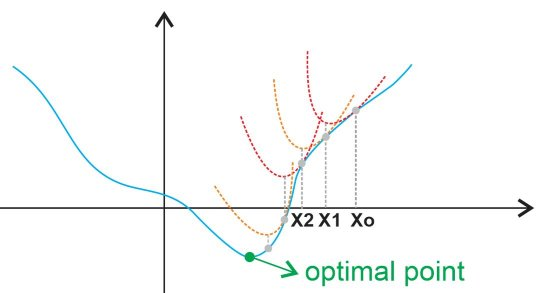
\includegraphics[width=1.2\linewidth]{pic/newton_ardianumam.jpg}
        \caption{\footnotesize Finding root using Taylor's expansion and Newton's method. Source: \href{https://ardianumam.wordpress.com}{Ardian Umam's Blog}}
    \end{figure}
\end{minipage}
\end{frame}

\begin{frame}{Newton's Method: Advantages and Disadvantages}
    \begin{itemize}
        \item Newton's method offers various benefits but also has limitations, especially in large-scale machine learning. Below is a summary:
    \end{itemize}
    \begin{table}[]
        \centering
        \small % Reduce font size
        \begin{tabular}{|c|c|}
            \hline
            \textbf{Advantages} & \textbf{Disadvantages} \\
            \hline
            \textbf{Faster Convergence} & \textbf{Computationally Expensive} \\
            Quadratic convergence enables reaching & Requires Hessian calculation, making it\\
            minima faster in convex problems. & costly in high-dimensional models. \\
            \hline
            \textbf{Adaptive Step Sizes} & \textbf{Memory Intensive} \\
            Curvature-based step adjustment avoids & Storing the Hessian matrix is memory-intensive\\
            slow progress in shallow regions. & for models with millions of parameters. \\
            \hline
            \textbf{Reduced Oscillations} & \textbf{Convergence Challenges} \\
            Curvature information stabilizes paths & May converge to saddle points in non-convex\\
            in oscillatory regions. & functions common in machine learning. \\
            \hline
        \end{tabular}
        \caption{Advantages and Disadvantages of Newton's Method}
    \end{table}
\end{frame}

% \section{References}
% \begin{frame}[allowframebreaks]
%     \bibliography{ref}
%     %\bibliographystyle{ieeetr}
%     \nocite{*} % used here because no citation happens in slides
%     % if there are too many try use:
%     \tiny\bibliographystyle{ieeetr}
% \end{frame}
\end{document}
